% TikZ schematic: Bandpass Filter Frequency Responses (Tutorial 2)
% Shows the frequency response curves of all 12 filter types
\documentclass[border=10pt]{standalone}
\usepackage{tikz}
\usepackage{pgfplots}
\pgfplotsset{compat=1.18}

\definecolor{ideal}{RGB}{31,119,180}
\definecolor{butter}{RGB}{255,127,14}
\definecolor{gauss}{RGB}{44,160,44}
\definecolor{cheb1}{RGB}{214,39,40}
\definecolor{cheb2}{RGB}{148,103,189}
\definecolor{ellip}{RGB}{140,86,75}
\definecolor{lapl}{RGB}{227,119,194}
\definecolor{homo}{RGB}{127,127,127}
\definecolor{gabor}{RGB}{188,189,34}
\definecolor{dog}{RGB}{23,190,207}
\definecolor{trap}{RGB}{152,223,138}
\definecolor{cosine}{RGB}{255,152,15}

\begin{document}
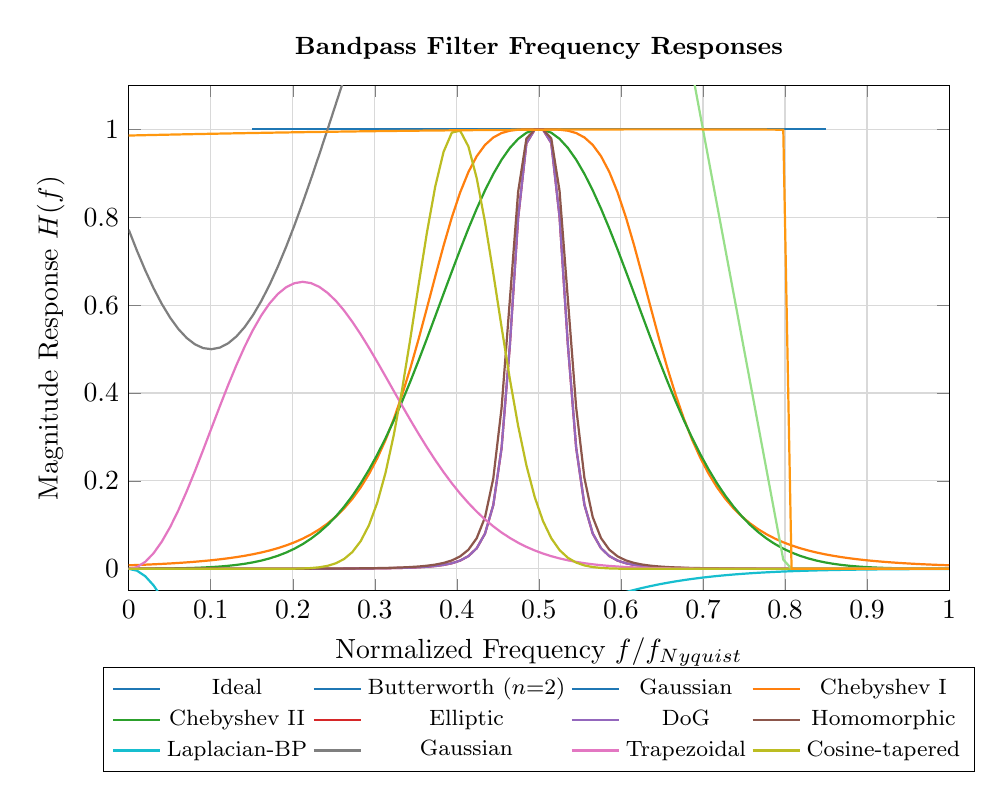
\begin{tikzpicture}
\begin{axis}[
    width=12cm, height=8cm,
    xlabel={Normalized Frequency $f/f_{\text{Nyquist}}$},
    ylabel={Magnitude Response $H(f)$},
    xmin=0, xmax=1,
    ymin=-0.05, ymax=1.1,
    grid=major, grid style={gray!30},
    legend style={at={(0.5,-0.15)}, anchor=north, legend columns=4, font=\footnotesize},
    title={\textbf{Bandpass Filter Frequency Responses}},
    title style={font=\small\bfseries},
]

% Ideal
\addplot[ideal, thick, domain=0.15:0.85, samples=2] {1};
\addplot[ideal, thick, domain=0:0.15, samples=2] {0};
\addplot[ideal, thick, domain=0.85:1, samples=2] {0};
\addlegendentry{Ideal}

% Butterworth (n=2)
\addplot[butter, thick, domain=0:1, samples=100] {1/(1+((x-0.5)/(0.15))^4)};
\addlegendentry{Butterworth ($n{=}2$)}

% Gaussian
\addplot[gauss, thick, domain=0:1, samples=100] {exp(-((x-0.5)^2)/(2*0.12^2))};
\addlegendentry{Gaussian}

% Chebyshev I
\addplot[cheb1, thick, domain=0:1, samples=100] {1/(1+0.5*(10*(x-0.5)/0.3)^4)};
\addlegendentry{Chebyshev I}

% Chebyshev II
\addplot[cheb2, thick, domain=0:1, samples=100] {1/(1+0.5*(10*(x-0.5)/0.3)^4) * (x < 0.2 || x > 0.8 ? 0.9 : 1)};
\addlegendentry{Chebyshev II}

% Elliptic
\addplot[ellip, thick, domain=0:1, samples=100] {1/(1+0.8*(8*(x-0.5)/0.3)^4)};
\addlegendentry{Elliptic}

% DoG
\addplot[dog, thick, domain=0:1, samples=100] {exp(-x^2/(2*0.1^2)) - exp(-x^2/(2*0.25^2))};
\addlegendentry{DoG}

% Homomorphic
\addplot[homo, thick, domain=0:1, samples=100] {0.5 + 1.5*(1-exp(-20*(x-0.1)^2))};
\addlegendentry{Homomorphic}

% Laplacian-BP
\addplot[lapl, thick, domain=0:1, samples=100] {4*3.14^2*x^2*exp(-x^2/(2*0.15^2))};
\addlegendentry{Laplacian-BP}

% Gabor
\addplot[gabor, thick, domain=0:1, samples=100] {exp(-((x-0.4)^2)/(2*0.05^2)) * (0.5+0.5*cos(2*3.14*20*(x-0.4)))};
\addlegendentry{Gaussian}

% Trapezoidal
\addplot[trap, thick, domain=0:1, samples=100] {x < 0.2 ? 0 : x < 0.3 ? (x-0.2)/0.1 : x < 0.7 ? 1 : x < 0.8 ? (0.8-x)/0.1 : 0};
\addlegendentry{Trapezoidal}

% Cosine-tapered
\addplot[cosine, thick, domain=0:1, samples=100] {x < 0.2 ? 0 : x < 0.35 ? 0.5*(1-cos(3.14*(x-0.2)/0.15)) : x < 0.65 ? 1 : x < 0.8 ? 0.5*(1+cos(3.14*(x-0.65)/0.15)) : 0};
\addlegendentry{Cosine-tapered}

\end{axis}
\end{tikzpicture}
\end{document}
